\chapter{Experimentación y Resultados}
    Aquí se presentaran los resultados del \textbf{Análisis a Priori y Posteriori} del algoritmo de rotación de imagen. 
    
\section{Algoritmo: Rotación Imagen}
    Rotación de Imagen consta de descomponer una imagen en su matriz RGB, donde se almacena toda la información de la imagen. Con esto se puede rotar el archivo haciendo uso de una función que invierta la posición de de los elementos de la matriz. El algoritmo se ejecutó de manera correcta, siendo capaz de rotar imágenes dividendo los sectores. En la figura \ref{fig:imgrotadas} se muestra una de las imágenes puestas de tamaño 100x100 a prueba por el algoritmo.

    \begin{figure}[!h]
        \centering
        
\includegraphics[width=5cm]{Images/Cat-test/orig100x100.png}\hfill
        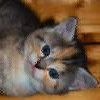
\includegraphics[width=5cm]{Images/Cat-test/result100x100.png}\hfill
        \caption{Imagen Rotada por Algoritmo}
        \label{fig:imgrotadas}
    \end{figure}

    \newpage
    \subsection{Análisis a Priori}
        La figura \ref{fig:priori} presenta el análisis a priori realizado sobre el pseudocódigo del algoritmo de Rotación de Imágenes. Concluyendo que el algoritmo presenta \(T(n) = 4T(\frac{n}{2}) + \theta(n)\)
        %\(f(n) = O(n)\)
        
        \begin{figure}[htp!]
            \centering
            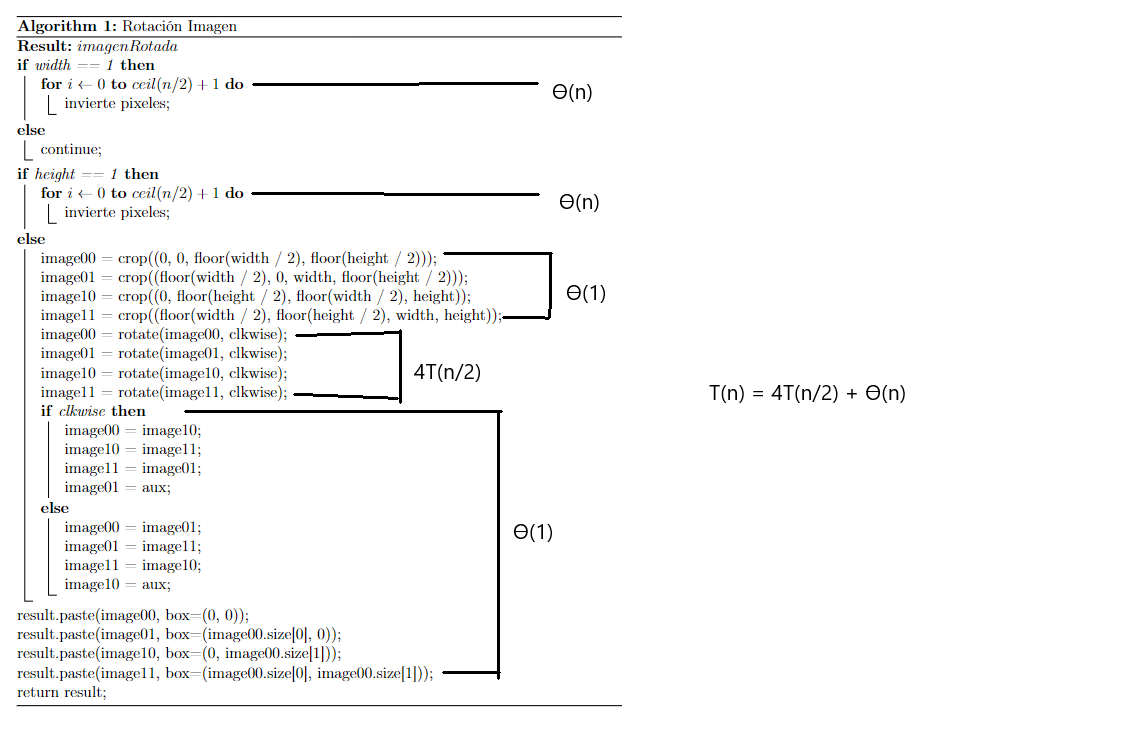
\includegraphics[width=1 \textwidth]{Images/A_Priori/priori.png}
            \caption{Análisis a Priori: Rotación Imagen}
            \label{fig:priori}
        \end{figure}

        \subsection{Desarrollo Análisis a Priori}
            Probando mediante el Teorema Maestro, resulta:
            Con \(T(n) = 4T(\frac{n}{2}) + \theta(n)\) se tiene \(a=4, b=2, f(n) = cn\)
            \newline
            Por el caso (III) del Teorema Maestro se obtiene un orden de complejidad de: 
                \begin{gather*}
                    \theta(n^{log_{2}4})\\
                    \therefore T(n)\in \theta(n^{2})
                    % \therefore  T(n)\in O(n)
                \end{gather*}
    
    
    \newpage    
    \subsection{Análisis a Posteriori}
        En el análisis posteriori se verifica que el análisis a priori demostró que la complejidad del peor caso es \(\theta(n^{2})\). En la figura \ref{fig:posteriori1} se muestra la función que acota al peor caso junto con los puntos que demuestran la complejidad del algoritmo funcionando de manera aleatoria y el mejor caso en el eje de las x siendo constante. 
        \begin{figure}[htp!]
            \centering
            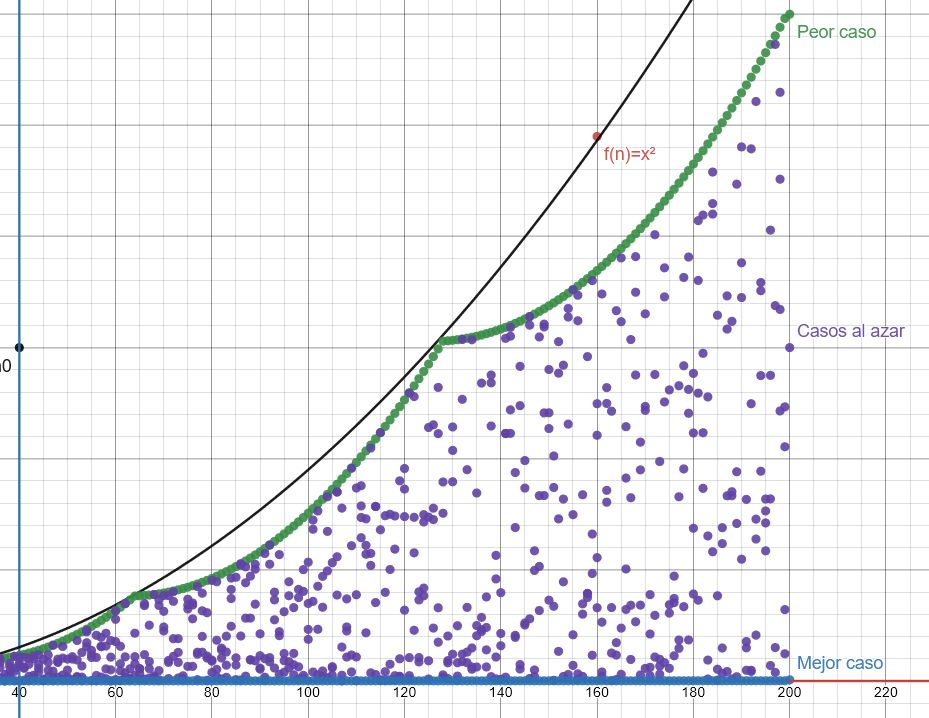
\includegraphics[width=1 \textwidth]{Images/A_Posteriori/posteriori.jpg}  
            \caption{Análisis a Posteriori: Rotación Imagen}
            \label{fig:posteriori1}
        \end{figure}
    
    
    
    \newpage
    \section{Pantallas de Ejecución del Algoritmo}
    Se muestra en la figura \ref{fig:rotas} la ejecución del algoritmo, haciendo uso de imágenes externas de diferente tamaños para medir el rendimiento tomando en cuenta diferentes imágenes de diferentes tamaños. 
    
        \begin{figure}[htp!]
            \centering
            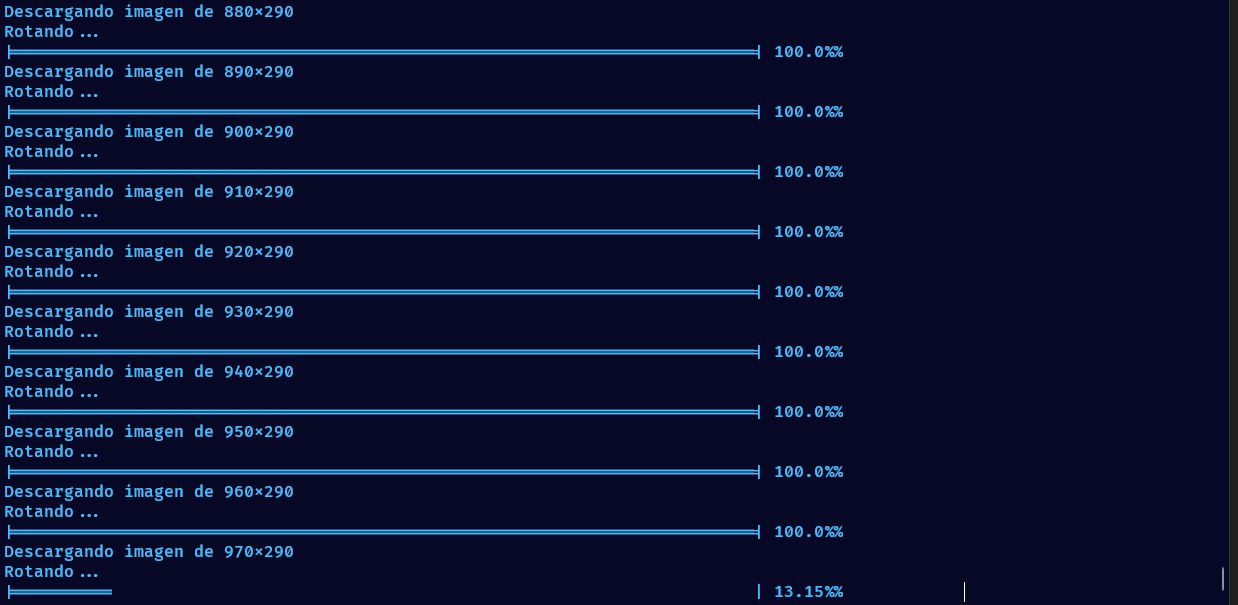
\includegraphics[width=0.8 \textwidth]{Images/Pantallas/ejecucion.jpg}  
            \caption{Ejecución de Rotación de Imagenes}
            \label{fig:rotas}
        \end{figure}
    